\documentclass{beamer}
%\documentclass[xcolor=dvipsnames]{beamer}
\usepackage[spanish]{babel}
\usepackage[utf8]{inputenc}
\usepackage{graphicx}
\usepackage{csquotes}
\usepackage{algorithm,algorithmic}
\usepackage[]{algorithm2e}
\usepackage{subfig}

\newcommand{\beamer}{\textsc{beamer}}
\newtheorem{definicion}{Definición}
\newtheorem{ejemplo}{Ejemplo}

%%%%%%%%%%%%%%%%%%%%%%%%%%%%%%%%%%%%%%%%%%%%%%%%%%%%%%%%%%%%%%%%%%%%%%%%%%%%%%%
\title[genetics.js]{
    genetics.js \\
    Framework web de computación evolutiva
}
\author[Cristian Abrante]{Cristian Manuel Abrante Dorta}
\institute[ULL]{Universidad de La Laguna}
\date[21-06-2019]{\today}
%%%%%%%%%%%%%%%%%%%%%%%%%%%%%%%%%%%%%%%%%%%%%%%%%%%%%%%%%%%%%%%%%%%%%%%%%%%%%%%

\usetheme{Madrid}
%\usetheme{Warsaw}

%%%%%%%%%%%%%%%%%%%%%%%%%%%%%%%%%%%%%%%%%%%%%%%%%%%%%%%%%%%%%%%%%%%%%%%%%%%%%%%
\definecolor{pantone254}{RGB}{87,6,140}
\definecolor{pantone3015}{RGB}{0,88,147}
\definecolor{pantone432}{RGB}{56,61,66}
\setbeamercolor*{palette primary}{use=structure,fg=white,bg=pantone254}
\setbeamercolor*{palette secondary}{use=structure,fg=white,bg=pantone3015}
\setbeamercolor*{palette tertiary}{use=structure,fg=white,bg=pantone432}
\setbeamercolor*{palette sidebar primary}{use=structure,fg=pantone254}
\setbeamercolor*{palette sidebar tertiary}{use=structure,fg=pantone3015}
\setbeamercolor*{block title}{bg=pantone3015,fg=white}
\setbeamercolor*{alerted text}{fg=pantone432}
\setbeamercolor*{item projected}{fg=pantone254}
\setbeamercolor*{section in toc shaded}{use=structure,fg=structure.fg}
\setbeamercolor*{section in toc}{fg=pantone3015}
\setbeamercolor*{subsection in toc shaded}{fg=pantone3015}
\setbeamercolor*{subsection in toc}{fg=pantone432}

%%%%%%%%%%%%%%%%%%%%%%%%%%%%%%%%%%%%%%%%%%%%%%%%%%%%%%%%%%%%%%%%%%%%%%%%%%%%%%%
\begin{document}
  
%++++++++++++++++++++++++++++++++++++++++++++++++++++++++++++++++++++++++++++++  
\begin{frame}

  
\includegraphics[width=0.45\textwidth]{pres/img/etsit-logo.png}
  \hspace*{2cm}
  
\includegraphics[width=0.35\textwidth]{pres/img/geneticsjs-logo.png}
  \titlepage

  \begin{scriptsize}
    \begin{center}
     Escuela Superior de Ingeniería y Tecnología \\
     Universidad de La Laguna
    \end{center}
  \end{scriptsize}

\end{frame}
%++++++++++++++++++++++++++++++++++++++++++++++++++++++++++++++++++++++++++++++  

%++++++++++++++++++++++++++++++++++++++++++++++++++++++++++++++++++++++++++++++  
\begin{frame}[allowframebreaks]
  \frametitle{Índice}  
  \tableofcontents[sections={1-3}]
  \framebreak
  \tableofcontents[sections={4-5}]
\end{frame}
%++++++++++++++++++++++++++++++++++++++++++++++++++++++++++++++++++++++++++++++  
% used to print plan before each section

\AtBeginSection[]
{
  \begin{frame}
    \frametitle{Índice}
    \tableofcontents[currentsection, hideallsubsections]
  \end{frame}
}

%++++++++++++++++++++++++++++++++++++++++++++++++++++++++++++++++++++++++++++++  

\section{Introducción}

%++++++++++++++++++++++++++++++++++++++++++++++++++++++++++++++++++++++++++++++  

\subsection{$\mathcal{P}$ vs $\mathcal{NP}$}

%++++++++++++++++++++++++++++++++++++++++++++++++++++++++++++++++++++++++++++++  
\begin{frame}
\frametitle{$\mathcal{P}$ vs $\mathcal{NP}$}

En primer lugar, veremos una clasificación de los problemas en función de su complejidad computacional.

\begin{figure}
    \centering
    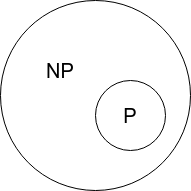
\includegraphics[scale=0.5]{pres/img/introduccion/p-np.png}
    \caption{Representación de las clases de problemas $\mathcal{P}$ y $\mathcal{NP}$}
    \label{fig:p-np}
\end{figure}

\begin{itemize}
    \item \textbf{Clase $\mathcal{P}$}: Se puede \textbf{encontrar} una solución en tiempo polinomial.
    \item \textbf{Clase $\mathcal{NP}$}: Se puede \textbf{verificar} una solución en tiempo polinomial.
\end{itemize}

\end{frame}
%++++++++++++++++++++++++++++++++++++++++++++++++++++++++++++++++++++++++++++++  

\subsection{Optimización combinatoria}

%++++++++++++++++++++++++++++++++++++++++++++++++++++++++++++++++++++++++++++++  
\begin{frame}
\frametitle{Optimización combinatoria}

Dentro de la clase $\mathcal{NP}$, existen una gran cantidad de problemas de \textbf{optimización combinatoria}.

\bigskip

\begin{block}{Optimización combinatoria}
 En este tipo de problemas, se trata de optimizar una función objetivo, que depende de una serie de variables \textbf{discretas}, sujetas a un conjunto de restricciones.
\end{block}

\bigskip

Algunos ejemplos de este tipo de problemas:

\begin{itemize}
    \item Problema del viajante de comercio (TSP).
    \item Problema de rutas de vehículos (VRP).
    \item Problema del vertext cover.
\end{itemize}
\end{frame}
%++++++++++++++++++++++++++++++++++++++++++++++++++++++++++++++++++++++++++++++

%++++++++++++++++++++++++++++++++++++++++++++++++++++++++++++++++++++++++++++++
\begin{frame}
\frametitle{Optimización combinatoria}

Formalmente, un problema ($P$) de optimización combinatoria se puede definir como una tupla:

\begin{center}
    $P = (S, f, \Omega)$
\end{center}

Donde:

\begin{itemize}
    \item \textbf{Espacio de soluciones} ($S$): Es el conjunto finito y numerable de todas las posibles soluciones al problema.
    \item \textbf{Función objetivo} ($f$): Para cada solución de $S$, devuelve su puntuación.
    \begin{center}
        \begin{math}
            f: S \rightarrow \mathbb{R}
        \end{math}
    \end{center}
    \item \textbf{Conjunto de restricciones} ($\Omega$): Conjunto de restricciones que debe satisfacer una solución de s ($s \in S$), para ser válida.
\end{itemize}

\end{frame}
%++++++++++++++++++++++++++++++++++++++++++++++++++++++++++++++++++++++++++++++

%++++++++++++++++++++++++++++++++++++++++++++++++++++++++++++++++++++++++++++++
\begin{frame}
\frametitle{Optimización combinatoria}

El concepto de \textbf{óptimo global} ($s^*$) es la solución para la cual la función objetivo tiene una evaluación más alta, en el caso de un problema de \textbf{maximización}:

\begin{center}
    $\forall s \in S, \quad f(s^*) \geq f(s)$ 
\end{center}

O mas baja en el caso de un problema de \textbf{minimización}:

\begin{center}
    $\forall s \in S, \quad f(s^*) \leq f(s)$ 
\end{center}

Para encontrar esta solución, existen varias opciones:

\begin{itemize}
    \item Enumerar todas las soluciones de $S$. Esto suele ser \textbf{inviable} debido al gran tamaño de este conjunto.
    \item Utilizar una \textbf{exploración inteligente} del espacio de soluciones. Utilizando por ejemplo, \textbf{metaheurísticas}.
\end{itemize}

\end{frame}
%++++++++++++++++++++++++++++++++++++++++++++++++++++++++++++++++++++++++++++++

\subsection{Metaheurísticas}

%++++++++++++++++++++++++++++++++++++++++++++++++++++++++++++++++++++++++++++++
\begin{frame}
\frametitle{Metaheurísticas}

\begin{block}{Metaheurísticas}
 Las metaheurísticas se centran en encontrar soluciones a problemas de optimización aplicando una búsqueda en el espacio de soluciones ($S$), cuando no se tiene información específica del problema.
\end{block}

\bigskip

Existen muchas técnicas metaheurísticas, que se pueden clasificar según diferentes criterios, sin embargo en este trabajo nos centraremos en la \textbf{computación evolutiva}.

\end{frame}
%++++++++++++++++++++++++++++++++++++++++++++++++++++++++++++++++++++++++++++++  

\section{Computación evolutiva}

%++++++++++++++++++++++++++++++++++++++++++++++++++++++++++++++++++++++++++++++  

\subsection{Definición}

%++++++++++++++++++++++++++++++++++++++++++++++++++++++++++++++++++++++++++++++  
\begin{frame}
\frametitle{Computación evolutiva}

\begin{exampleblock}{}
  {\large ``La gran ventaja de la evolución es la gran cantidad de especies diferentes que ha creado, cada una adaptada a su medio''}
  \vskip5mm
  \hspace*\fill{\small--- A.E. Eiben y J.E. Smith}
\end{exampleblock}

\begin{block}{Computación evolutiva}
 La \textbf{computación evolutiva} es una técnica metaheurística, bio-inpirada y basada en población. Utilizada para resolver diversos problemas complejos, y especialmente útil a la hora de resolver problemas de \textbf{optimización combinatoria}.
\end{block}

\end{frame}
%++++++++++++++++++++++++++++++++++++++++++++++++++++++++++++++++++++++++++++++  

\subsection{Historia}

%++++++++++++++++++++++++++++++++++++++++++++++++++++++++++++++++++++++++++++++  
\begin{frame}
\frametitle{Historia}

\begin{columns}
\column{0.5\textwidth}
La inspiración principal de la computación evolutiva es la \textbf{Teoría de la evolución de Darwin}. En la cual se exponen conceptos clave como la \textbf{selección natural} o la \textbf{supervivencia de los individuos más adaptados}.

\column{0.5\textwidth}
\begin{figure}
    \centering
    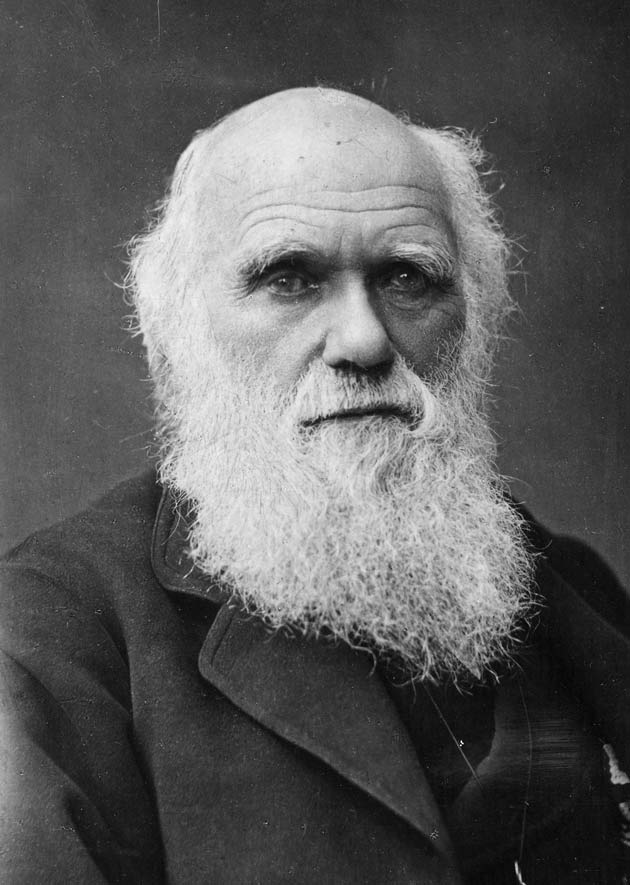
\includegraphics[scale=0.15]{pres/img/darwin.jpg}
    \caption{Charles Darwin}
    \label{fig:darwin}
\end{figure}
\end{columns}

\end{frame}
%++++++++++++++++++++++++++++++++++++++++++++++++++++++++++++++++++++++++++++++

%++++++++++++++++++++++++++++++++++++++++++++++++++++++++++++++++++++++++++++++  
\begin{frame}
\frametitle{Historia}

El desarrollo de la computación evolutiva se produce a partir de los \textbf{años sesenta}:

\begin{description}
    \item[1962] Bremermann ejecuta el primer experimento sobre \textbf{Optimización mediante evolución y recombinación}.
    \item[1965] Fogel, Owen y Walsh introducen el término de \textbf{Programación evolutiva}.
    \item[1973] Holland desarrolla los \textbf{algoritmos genéticos}.
    \item[1973] Rechenberg y Schwefel crean las \textbf{estrategias evolutivas}.
    \item[1990] Se unifican todos los conceptos, definiendo el término \textbf{computación evolutiva}
\end{description}

\end{frame}
%++++++++++++++++++++++++++++++++++++++++++++++++++++++++++++++++++++++++++++++  

\subsection{Estructura}

%++++++++++++++++++++++++++++++++++++++++++++++++++++++++++++++++++++++++++++++  
\begin{frame}
\frametitle{Estructura}

La estructura de un algoritmo evolutivo es la siguiente:

\begin{algorithm}[H]
 INICIALIZAR la población con $n$ individuos aleatorios;\\
 EVALUACIÓN de la población mediante la función de puntuación (\textit{fitness});
 
 \While{CONDICIÓN DE PARADA no sea satisfecha}{
  SELECCIÓN de padres; \\
  RECOMBINACIÓN de pares de padres; \\
  MUTACIÓN de la descendencia; \\
  EVALUACIÓN de la descendencia; \\
  SELECCIÓN de supervivientes para la siguiente generación;
 }
 \caption{Esquema básico de un algoritmo evolutivo}
\end{algorithm}

\end{frame}
%++++++++++++++++++++++++++++++++++++++++++++++++++++++++++++++++++++++++++++++  

%++++++++++++++++++++++++++++++++++++++++++++++++++++++++++++++++++++++++++++++ 
\begin{frame}
\frametitle{Estructura}

Los algoritmos evolutivos permiten realizar una exploración inteligente del espacio de soluciones ($S$) del problema gracias a:

\bigskip

\begin{itemize}
    \item \textbf{Variación}: Las fases de mutación y recombinación garantizan la diversidad en las soluciones.
    \item \textbf{Intensificación}: Las fases de selección de padres y descendencia, garantizan que se evaluen las mejores soluciones.
\end{itemize}

\end{frame}
%++++++++++++++++++++++++++++++++++++++++++++++++++++++++++++++++++++++++++++++

\section{Objetivos}

%++++++++++++++++++++++++++++++++++++++++++++++++++++++++++++++++++++++++++++++

\subsection{Bibliotecas de algoritmos evolutivos}

%++++++++++++++++++++++++++++++++++++++++++++++++++++++++++++++++++++++++++++++ 
\begin{frame}
\frametitle{Bibliotecas de algoritmos evolutivos}

Existen numerosas bibliotecas de algoritmos evolutivos, que contienen una implementación de los métodos más comunes existentes en cada fase. \\

\bigskip

\begin{itemize}
    \item \textbf{Desarrolladas en Java}: Opt4J, Optimization Algorithm Toolkit, JMetal, ...
    \item \textbf{Desarrolladas en C++}: ParadisEO, METCO,..
\end{itemize}

\bigskip

Se ha identificado la carencia de un \textit{framework} de este propósito, pero \textbf{orientado a aplicaciones web}.

\end{frame}
%++++++++++++++++++++++++++++++++++++++++++++++++++++++++++++++++++++++++++++++

\subsection{Objetivos}

%++++++++++++++++++++++++++++++++++++++++++++++++++++++++++++++++++++++++++++++ 
\begin{frame}
\frametitle{Objetivos}

\begin{block}{Desarrollo}
 El objetivo de este proyecto es el desarrollo de \textbf{genetics.js}, un \textit{framework} que contenga los principales métodos que cubran todas las fases de un algoritmo evolutivo.
\end{block}

\bigskip

Además debe cumplir los siguientes criterios:

\begin{itemize}
    \item Garantizar la compatibilidad con aplicaciones web.
    \item Estar implementado en un lenguaje de programación moderno y soportado por la comunidad.
    \item Utilizar herramientas que garanticen la continuidad del proyecto.
    \item Contar con una buena documentación.
    \item Garantizar que pueda ser extensible.
\end{itemize}

\end{frame}
%++++++++++++++++++++++++++++++++++++++++++++++++++++++++++++++++++++++++++++++

\subsection{Roadmap}

%++++++++++++++++++++++++++++++++++++++++++++++++++++++++++++++++++++++++++++++ 
\begin{frame}
\frametitle{Objetivos}

Para cumplir estos criterios y objetivos se ha elaborado un \textbf{Roadmap} basado en \textbf{semantic versioning}:

\bigskip

\begin{itemize}
    \item \texttt{0.1.0}: Implementación de la codificación de soluciones mediante individuos.
    \item \texttt{0.2.0}: Implementación de los operadores de mutación.
    \item \texttt{0.3.0}: Impelementación de los operadores de cruce.
    \item \texttt{0.4.0}: Implementación de los operadores de selección de padres. 
    \item \texttt{0.5.0}: Implementación de los operadores de selección de supervivientes.
    \item \texttt{0.6.0}: Implementación de las clases gestoras de la población de individuos.
\end{itemize}

\end{frame}
%++++++++++++++++++++++++++++++++++++++++++++++++++++++++++++++++++++++++++++++

\section{Desarrollo}

%++++++++++++++++++++++++++++++++++++++++++++++++++++++++++++++++++++++++++++++ 

\subsection{Tecnologías utilizadas}

%++++++++++++++++++++++++++++++++++++++++++++++++++++++++++++++++++++++++++++++ 
\begin{frame}
\frametitle{Tecnologías utilizadas}

Dado que la biblioteca debe ser completamente compatible con aplicaciones web, lo más lógico es desarrollarla con el \textit{stack} del lenguaje \textbf{JavaScript}.

\begin{figure}
    \centering
    \subfloat{
\includegraphics[width=2cm]{mem/images/cap-4/4.1.1(JS)/js-logo.png}}
    \qquad
    \subfloat{
\includegraphics[width=3cm]{mem/images/cap-4/4.1.1(JS)/node-logo.png}}
    \qquad
    \subfloat{
\includegraphics[width=3cm]{mem/images/cap-4/4.1.1(JS)/npm-logo.png}}
    \caption{Logos de JavaScript, Node y NPM}
    \label{fig:1}
\end{figure}

Distinguiremos entre tecnologías utilizadas \textbf{durante el desarrollo} y dependencias en \textbf{producción}.

\end{frame}
%++++++++++++++++++++++++++++++++++++++++++++++++++++++++++++++++++++++++++++++

\subsubsection{Tecnologías utilizadas en el desarrollo}

%++++++++++++++++++++++++++++++++++++++++++++++++++++++++++++++++++++++++++++++ 
\begin{frame}
\frametitle{Tecnologías utilizadas en el desarrollo}

El lenguaje de programación utilizado para el desarrollo ha sido \textbf{TypeScript}:

\medskip

\begin{figure}
    \centering
    
\includegraphics[scale=0.1]{mem/images/cap-4/4.1.2(desarrollo)/typescript-logo.png}
    \caption{Logo de TypeScript}
    \label{fig:typescript}
\end{figure}

\medskip

La utilización de este lenguaje aporta ciertas ventajas frente a \textbf{JavaScript}, como seguridad de tipos, y escalabilidad. 

\end{frame}
%++++++++++++++++++++++++++++++++++++++++++++++++++++++++++++++++++++++++++++++

%++++++++++++++++++++++++++++++++++++++++++++++++++++++++++++++++++++++++++++++ 
\begin{frame}
\frametitle{Tecnologías utilizadas en el desarrollo}

Para garantizar la continuidad, estabilidad y calidad del software se han utilizado las siguientes herramientas:

\begin{figure}
    \centering
    \subfloat{
\includegraphics[scale=0.16]{mem/images/cap-4/4.1.2(desarrollo)/typedoc-logo.png}}
    \qquad
    \subfloat{
\includegraphics[scale=0.16]{mem/images/cap-4/4.1.2(desarrollo)/jest-logo.png}}
    \qquad
    \subfloat{
\includegraphics[scale=0.1]{mem/images/cap-4/4.1.2(desarrollo)/circleci-logo.png}}
    \qquad
    \subfloat{
\includegraphics[scale=0.15]{mem/images/cap-4/4.1.2(desarrollo)/coveralls-logo.png}}
    \caption{Logos de TypeDoc, Jest, CricleCI y Coveralls}
    \label{fig:1}
\end{figure}

\begin{itemize}
    \item \textbf{Documentación}: Se ha usado \textbf{TypeDoc}.
    \item \textbf{Tests}: Se ha utilizado \textbf{Jest}.
    \item \textbf{Integración contínua}: Se ha usado \textbf{CircleCI}.
    \item \textbf{Coverage}: Se ha elegido \textbf{Coveralls}.
\end{itemize}

\end{frame}
%++++++++++++++++++++++++++++++++++++++++++++++++++++++++++++++++++++++++++++++

%++++++++++++++++++++++++++++++++++++++++++++++++++++++++++++++++++++++++++++++ 
\begin{frame}
\frametitle{Tecnologías utilizadas en el desarrollo}

Para formatear el código y depurar los posibles errores he utilizado:

\begin{figure}
    \centering
    \subfloat{
\includegraphics[scale=0.025]{mem/images/cap-4/4.1.2(desarrollo)/prettier-logo.png}}
    \qquad
    \subfloat{
\includegraphics[scale=0.36]{mem/images/cap-4/4.1.2(desarrollo)/tslint-logo.png}}
    \qquad
    \subfloat{
\includegraphics[scale=0.1]{mem/images/cap-4/4.1.2(desarrollo)/webstorm-logo.png}}
    \caption{Logos de Prettier, ts-lint y WebStorm}
    \label{fig:1}
\end{figure}

\begin{itemize}
    \item \textbf{Prettier}: herramienta utilizada para formatear el código de manera común.
    \item \textbf{ts-lint}: Utilizado para comprobar errores de formato y de código antes de realizar la compilación.
    \item \textbf{WebStorm}: IDE utilizado para el desarrollo.
\end{itemize}

\end{frame}
%++++++++++++++++++++++++++++++++++++++++++++++++++++++++++++++++++++++++++++++

\subsubsection{Tecnologías utilizadas en producción}

%++++++++++++++++++++++++++++++++++++++++++++++++++++++++++++++++++++++++++++++ 
\begin{frame}
\frametitle{Tecnologías utilizadas en producción}

La intención es construir un \textbf{framework minimalista}, de tal forma que se tengan las mínimas dependencias posibles en producción.

\begin{center}
    \Huge \texttt{random.js}
\end{center}

\bigskip

Esta biblioteca se ha utilizado para llevar a cabo la \textbf{generación de números aleatorios}, pues nos permite entre otras cosas establecer la semilla con la que se generarán estos valores.

\end{frame}
%++++++++++++++++++++++++++++++++++++++++++++++++++++++++++++++++++++++++++++++

\subsection{Estructura del software}

%++++++++++++++++++++++++++++++++++++++++++++++++++++++++++++++++++++++++++++++ 
\begin{frame}
\frametitle{Estructura del software}

El desarrollo de \textbf{genetics.js} se ha hecho como un \textbf{paquete npm}.

\begin{figure}
    \centering
    
\includegraphics[scale=0.2]{pres/img/geneticsjs-logo.png}
    \caption{Logo de genetics.js}
    \label{fig:my_label}
\end{figure}

Los diferentes módulos que compondrán el software desarrollado se corresponden con los métodos más comunes para implementar las diferentes fases de los algoritmos evolutivos. 

\end{frame}
%++++++++++++++++++++++++++++++++++++++++++++++++++++++++++++++++++++++++++++++

%++++++++++++++++++++++++++++++++++++++++++++++++++++++++++++++++++++++++++++++ 
\begin{frame}
\frametitle{Individuos}

En los algoritmos evolutivos, los individuos de la población se corresponden con las \textbf{diferentes soluciones que puede tener el problema} que estemos resolviendo.

\begin{figure}
    \centering
    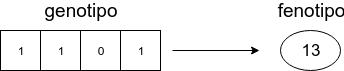
\includegraphics[scale=0.6]{mem/images/cap-4/4.2.2(Individuos)/Individuos-1.png}
    \caption{Ejemplo de conversión entre genotipo y fenotipo}
    \label{fig:ejemplo-1}
\end{figure}

\begin{itemize}
    \item \textbf{genotipo}: codificación de la solución que posee el individuo.
    \item \textbf{fenotipo}: valor que se le asocia a dicha codificación.
\end{itemize}

\end{frame}
%++++++++++++++++++++++++++++++++++++++++++++++++++++++++++++++++++++++++++++++ 

%++++++++++++++++++++++++++++++++++++++++++++++++++++++++++++++++++++++++++++++ 
\begin{frame}
\frametitle{Individuos}

\begin{columns}
    \column{0.5\textwidth}
    \begin{figure}
        \centering
        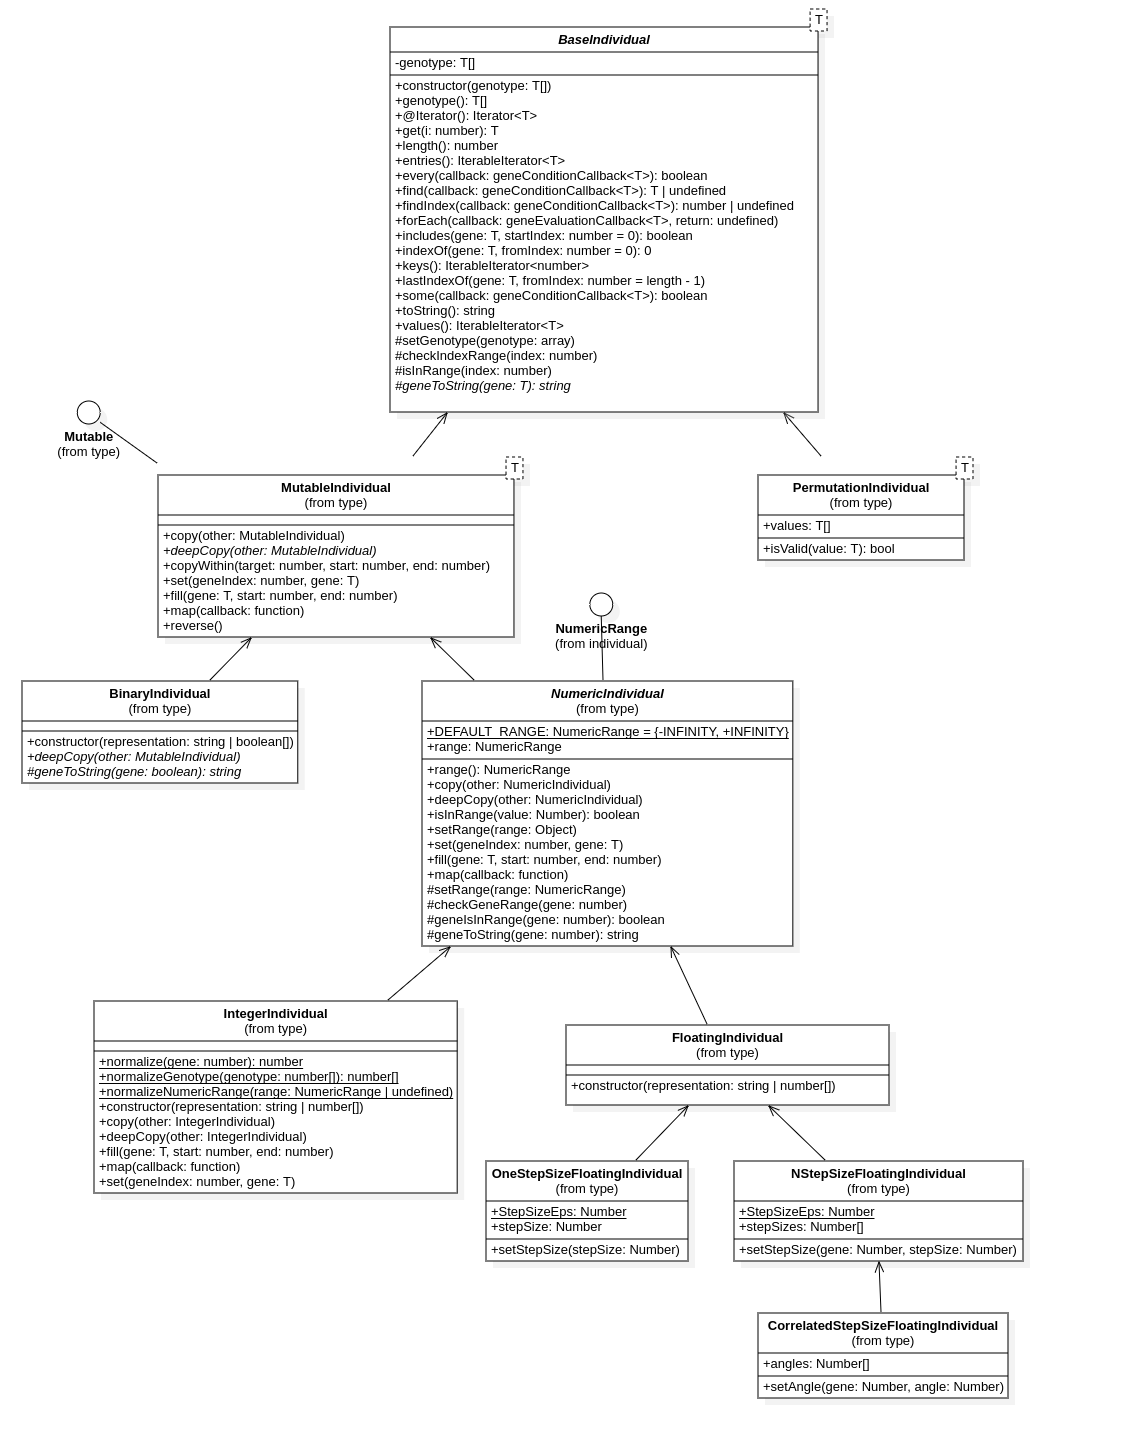
\includegraphics[scale=0.13]{mem/images/cap-4/4.2.2(Individuos)/Individual.png}
        \caption{Diagrama UML de los individuos}
        \label{fig:my_label}
    \end{figure}
    \column{0.5\textwidth}
    Los diferentes individuos implementados han sido:
    \begin{itemize}
        \item \texttt{BaseIndividual}
        \item \texttt{MutableIndividual}
        \item \texttt{BinaryIndividual}
        \item \texttt{NumericIndividual}
        \item \texttt{IntegerIndividual}
        \item \texttt{FloatingIndividual}
    \end{itemize}
\end{columns}

\end{frame}
%++++++++++++++++++++++++++++++++++++++++++++++++++++++++++++++++++++++++++++++ 

%++++++++++++++++++++++++++++++++++++++++++++++++++++++++++++++++++++++++++++++ 
\begin{frame}
\frametitle{Individuos}

\begin{figure}
  \centering
  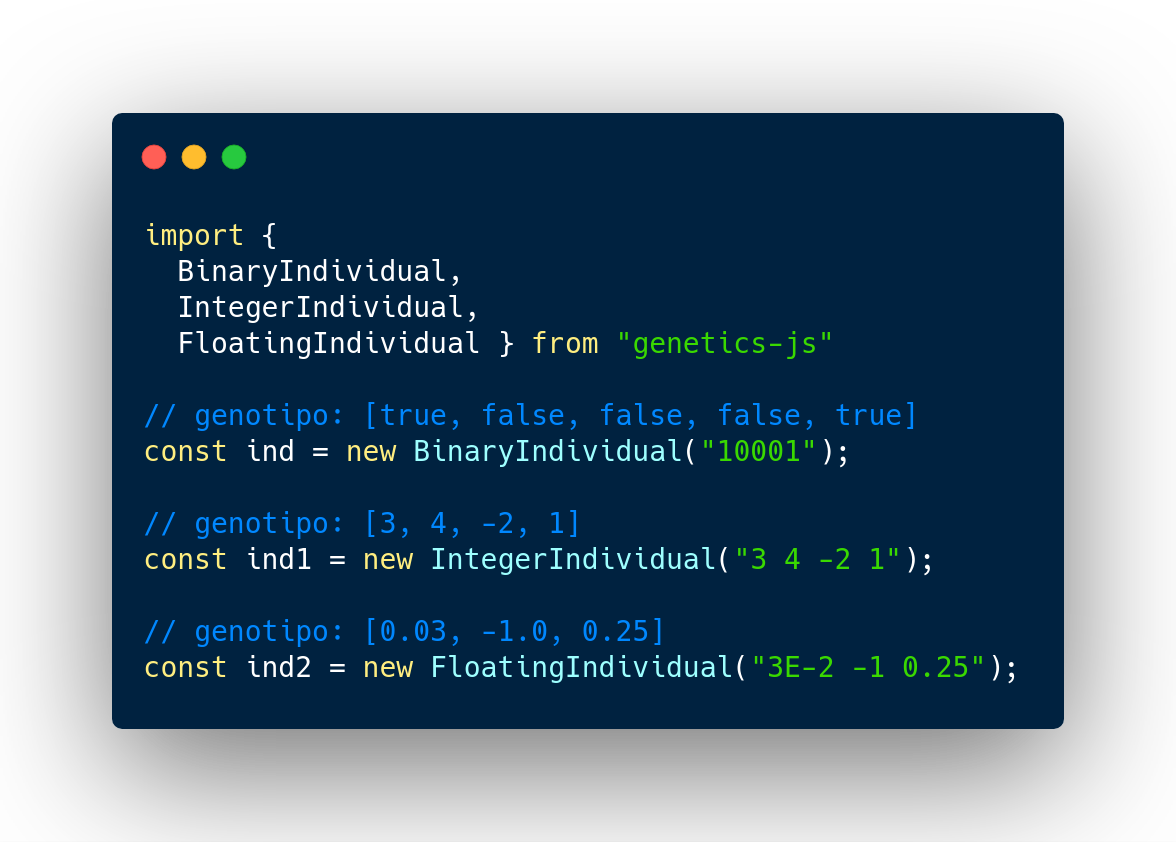
\includegraphics[scale=0.23]{pres/img/desarrollo/individual-example.png}
  \caption{Ejemplo de instanciación de diferentes individuos}
  \label{fig:my_label}
\end{figure}

\end{frame}
%++++++++++++++++++++++++++++++++++++++++++++++++++++++++++++++++++++++++++++++ 

%++++++++++++++++++++++++++++++++++++++++++++++++++++++++++++++++++++++++++++++ 
\begin{frame}
\frametitle{Generador de individuos}

El generador de individuos se utiliza para inicializar aleatoriamente la población.

\bigskip

\begin{columns}
    \column{0.6\textwidth}
    \begin{figure}
        \centering
        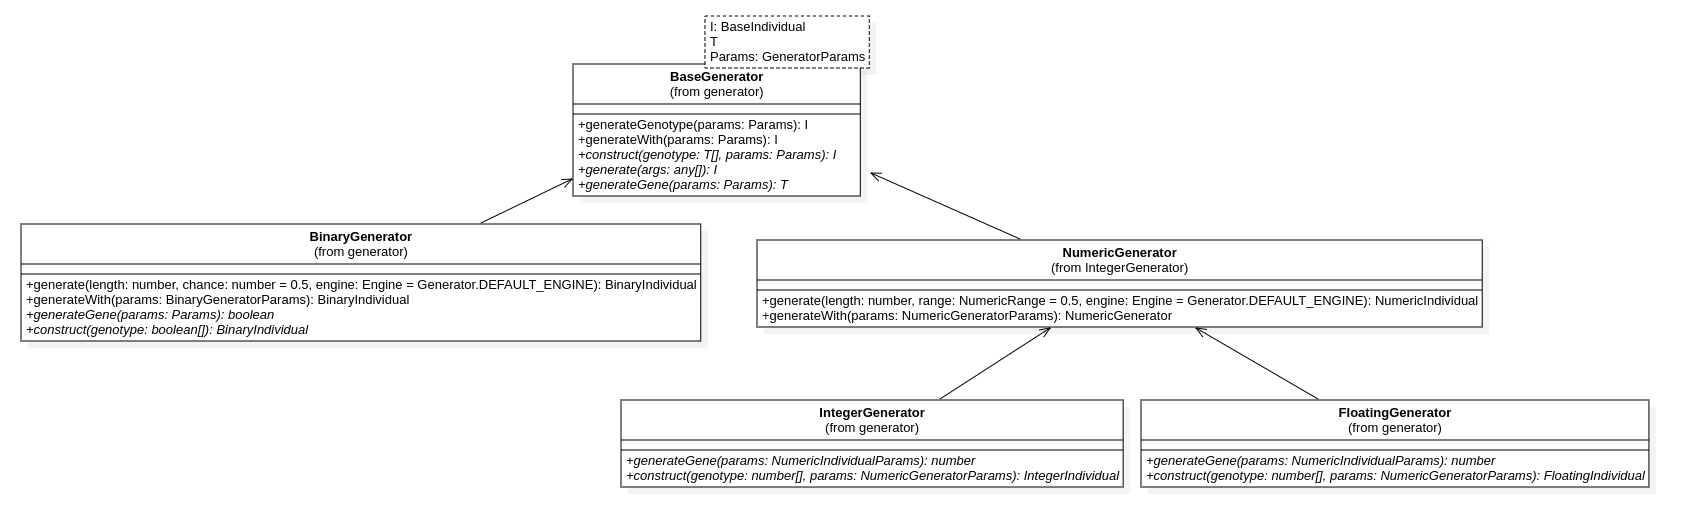
\includegraphics[scale=0.13]{mem/images/cap-4/4.2.3(Generador)/Generator.png}
        \caption{Diagrama UML del generador aleatorio}
        \label{fig:my_label}
    \end{figure}
    \column{0.4\textwidth}
    Los diferentes generadores implementados han sido:
    \begin{itemize}
        \item \texttt{BaseGenerator}
        \item \texttt{BinaryGenerator}
        \item \texttt{NumericGenerator}
        \item \texttt{IntegerGenerator}
        \item \texttt{FloatingGenerator}
    \end{itemize}
    
\end{columns}

\end{frame}
%++++++++++++++++++++++++++++++++++++++++++++++++++++++++++++++++++++++++++++++ 

%++++++++++++++++++++++++++++++++++++++++++++++++++++++++++++++++++++++++++++++ 
\begin{frame}
\frametitle{Generador de individuos}

\begin{figure}
    \centering
    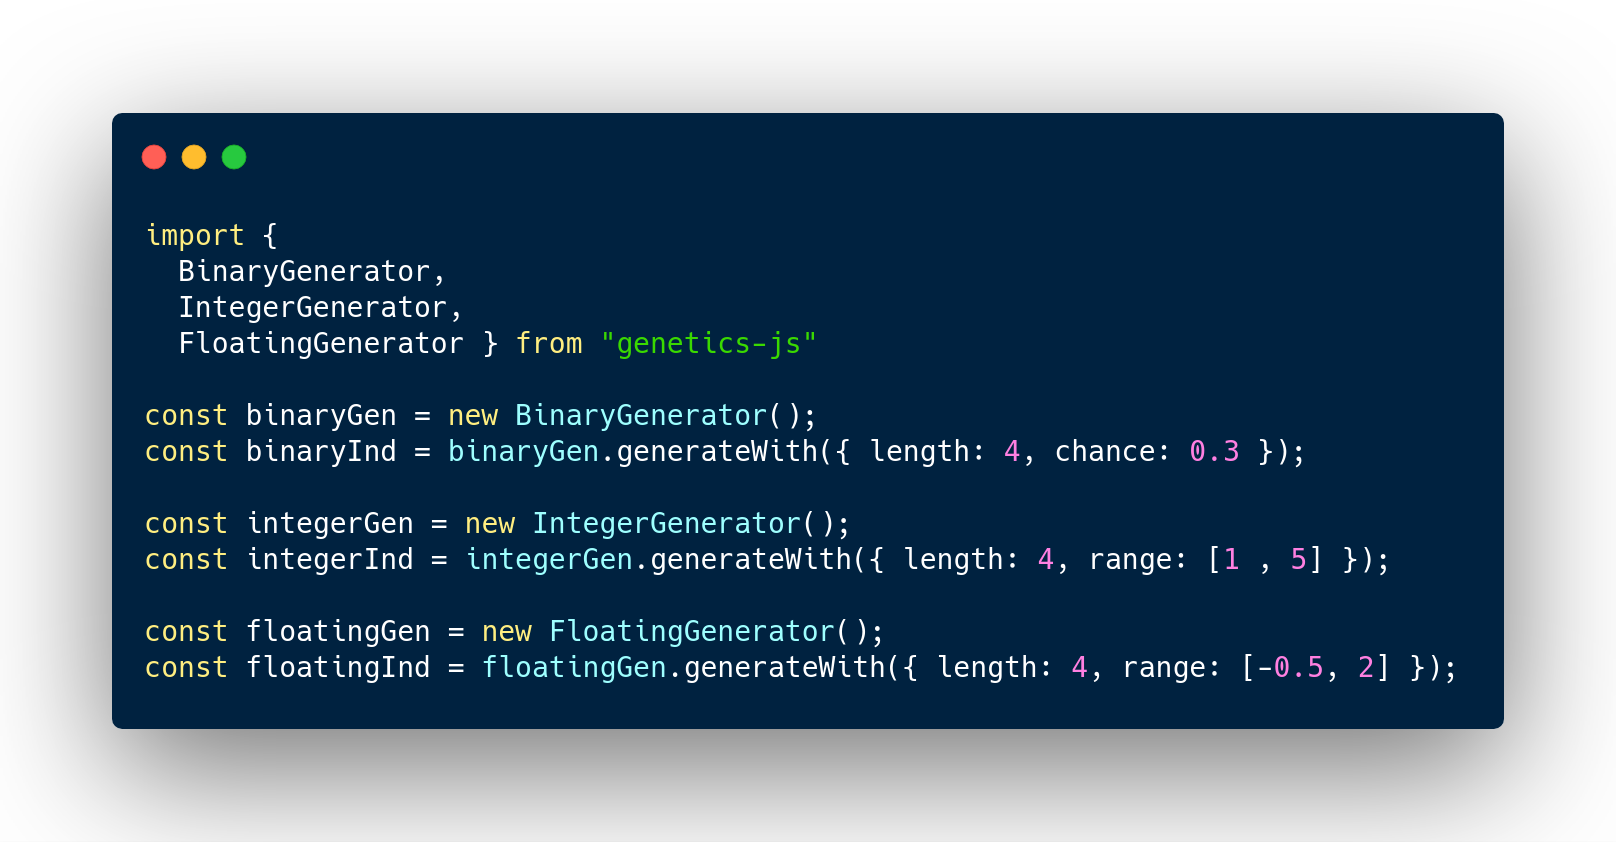
\includegraphics[scale=0.21]{pres/img/desarrollo/generator-example.png}
    \caption{Ejemplo de uso de diferentes generadores de individuos}
    \label{fig:my_label}
\end{figure}

\end{frame}
%++++++++++++++++++++++++++++++++++++++++++++++++++++++++++++++++++++++++++++++ 

%++++++++++++++++++++++++++++++++++++++++++++++++++++++++++++++++++++++++++++++ 
\begin{frame}
\frametitle{Gestión de la población}

La clase \texttt{Population} se utiliza para gestionar la población de individuos que compone nuestro problema.

\bigskip

\begin{columns}
    \column{0.5\textwidth}
    \begin{figure}
        \centering
        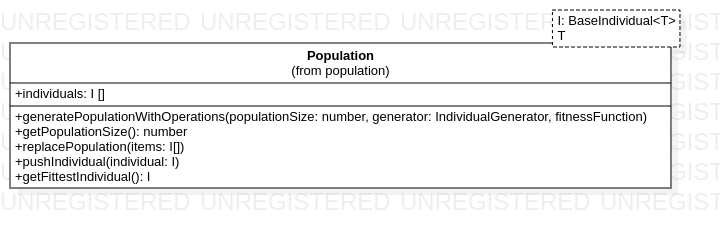
\includegraphics[scale=0.2]{mem/images/cap-4/4.2.4(Population)/Population.png}
        \caption{Diagrama UML de la clase \texttt{Population}}
        \label{fig:my_label}
    \end{figure}
    \column{0.5\textwidth}
    Los diferentes parámetros a los que se puede acceder son:
    \begin{itemize}
        \item \texttt{averageAge}
        \item \texttt{averageFitness}
        \item \texttt{fitnessSum}
        \item \texttt{fittestIndividualIndex}
    \end{itemize}
\end{columns}

\end{frame}
%++++++++++++++++++++++++++++++++++++++++++++++++++++++++++++++++++++++++++++++ 

%++++++++++++++++++++++++++++++++++++++++++++++++++++++++++++++++++++++++++++++ 
\begin{frame}
\frametitle{Selección de padres}

La fase de selección de padres consiste en seleccionar que individuos serán los que se \textbf{reproducirán para formar la descendencia}.

\bigskip

\begin{figure}
    \centering
    \subfloat{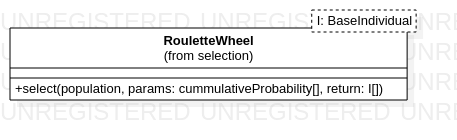
\includegraphics[scale=0.37]{mem/images/cap-4/4.2.5(Selection)/RouletteWheel.png}}
    \qquad
    \subfloat{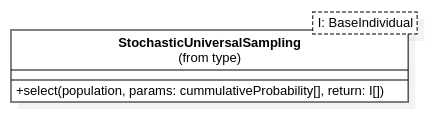
\includegraphics[scale=0.37]{mem/images/cap-4/4.2.5(Selection)/SUS.png}}
    \caption{Diagramas de \texttt{RouletteWheel} y \texttt{StochasticUniversalSampling}}
    \label{fig:1}
\end{figure}

Los métodos de selección implementados han sido:

\begin{itemize}
    \item \texttt{RouletteWheel}
    \item \texttt{StochasticUniversalSampling}
\end{itemize}

\end{frame}
%++++++++++++++++++++++++++++++++++++++++++++++++++++++++++++++++++++++++++++++

%++++++++++++++++++++++++++++++++++++++++++++++++++++++++++++++++++++++++++++++ 
\begin{frame}
\frametitle{Selección de padres}

\begin{figure}
    \centering
    \subfloat[Esquema del procedimiento Roulette Wheel]{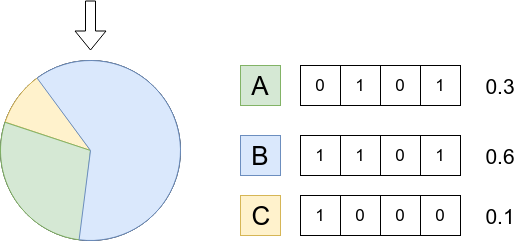
\includegraphics[scale=0.27]{mem/images/cap-4/4.2.5(Selection)/RouletteWheel-1.png}}
    \qquad
    \subfloat[Esquema del procedimiento Stochastic Universal Sampling]{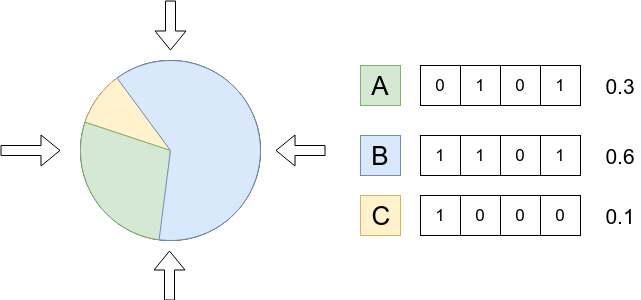
\includegraphics[scale=0.27]{mem/images/cap-4/4.2.5(Selection)/SUS-1.png}}
    \label{fig:1}
\end{figure}

\end{frame}
%++++++++++++++++++++++++++++++++++++++++++++++++++++++++++++++++++++++++++++++ 

%++++++++++++++++++++++++++++++++++++++++++++++++++++++++++++++++++++++++++++++ 
\begin{frame}
\frametitle{Operaciones de cruce}

Las operaciones de cruce consisten en generar una descendencia a partir de \textbf{dos individuos padres}.

\bigskip

\begin{columns}
    \column{0.4\textwidth}
    \begin{figure}
        \centering
        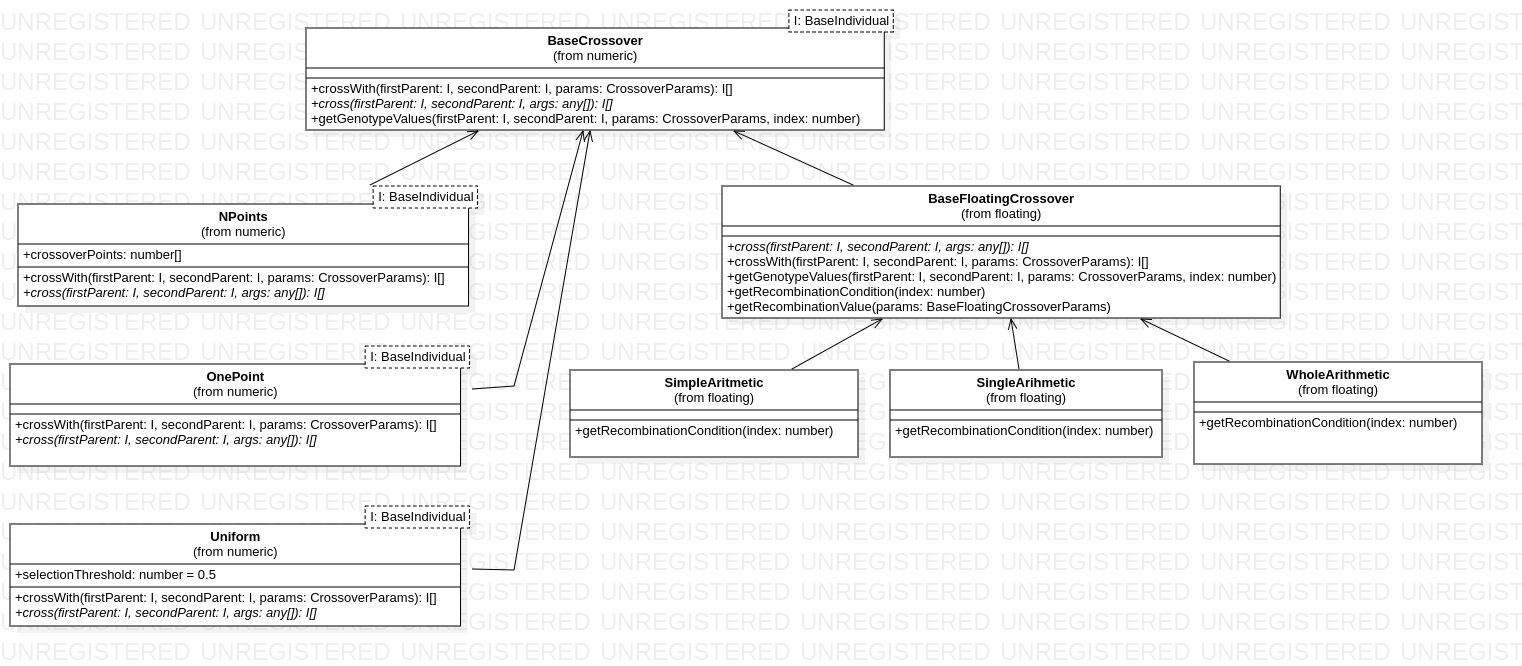
\includegraphics[scale=0.1]{mem/images/cap-4/4.2.6(Crossover)/Crossover.png}
        \caption{Diagrama UML de las operaciones de cruce}
        \label{fig:my_label}
    \end{figure}
    \column{0.6\textwidth}
    Los métodos que se han implementado han sido:
    \begin{itemize}
        \item \texttt{BaseCrossover} e interfaz \texttt{Crossover}
        \item \texttt{NPointsCrossover}
        \item \texttt{OnePointCrossover}
        \item \texttt{UniformCrossover}
        \item \texttt{SimpleArithmeticRecombination}
        \item \texttt{SingleArithmeticRecombination}
        \item \texttt{WholeArithmeticRecombination}
    \end{itemize}
\end{columns}

\end{frame}
%++++++++++++++++++++++++++++++++++++++++++++++++++++++++++++++++++++++++++++++

%++++++++++++++++++++++++++++++++++++++++++++++++++++++++++++++++++++++++++++++ 
\begin{frame}
\frametitle{Operaciones de cruce}

\begin{figure}
    \centering
    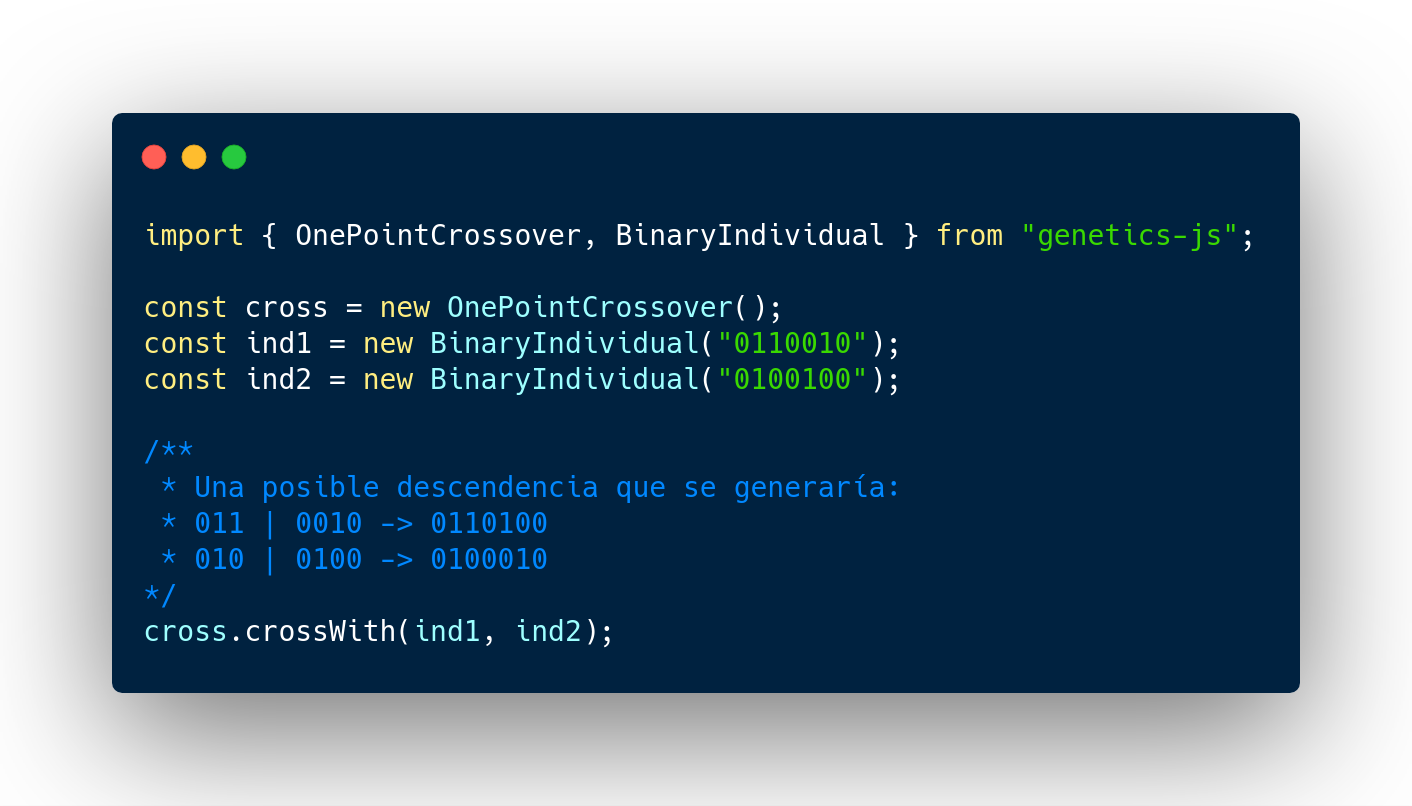
\includegraphics[scale=0.23]{pres/img/desarrollo/crossover-example.png}
    \caption{Ejemplo de una operación de cruce}
    \label{fig:my_label}
\end{figure}

\end{frame}
%++++++++++++++++++++++++++++++++++++++++++++++++++++++++++++++++++++++++++++++ 

%++++++++++++++++++++++++++++++++++++++++++++++++++++++++++++++++++++++++++++++ 
\begin{frame}
\frametitle{Operaciones de mutación}

Las operaciones de mutación tratan de \textbf{producir una cierta variación} en la descendencia generada mediante un operador de cruce.

\bigskip

\begin{columns}
    \column{0.47\textwidth}
    \begin{figure}
        \centering
        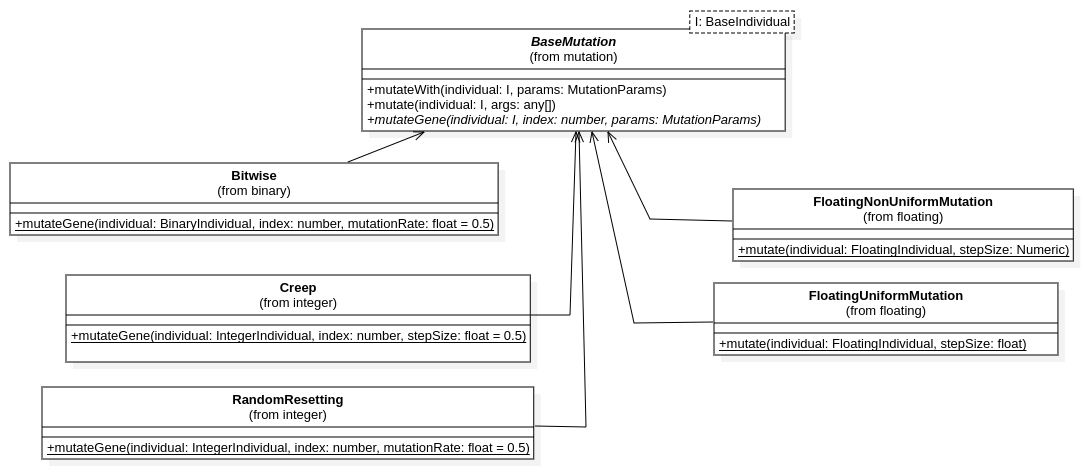
\includegraphics[width=\textwidth]{mem/images/cap-4/4.2.7(Mutation)/Mutation.png}
        \caption{Diagrama UML de las operaciones de mutación}
        \label{fig:my_label}
    \end{figure}
    \column{0.53\textwidth}
    Los métodos que se han implementado han sido:
    \begin{itemize}
        \item \texttt{MutationBase} e interfaz \texttt{Mutation}
        \item \texttt{BitwiseMutation}
        \item \texttt{CreepMutation}
        \item \texttt{RandomResetting}
        \item \texttt{FloatingNonUniformMutation}
        \item \texttt{FloatingUniformMutation}
    \end{itemize}
\end{columns}

\end{frame}
%++++++++++++++++++++++++++++++++++++++++++++++++++++++++++++++++++++++++++++++

%++++++++++++++++++++++++++++++++++++++++++++++++++++++++++++++++++++++++++++++ 
\begin{frame}
\frametitle{Operaciones de mutación}

\begin{figure}
    \centering
    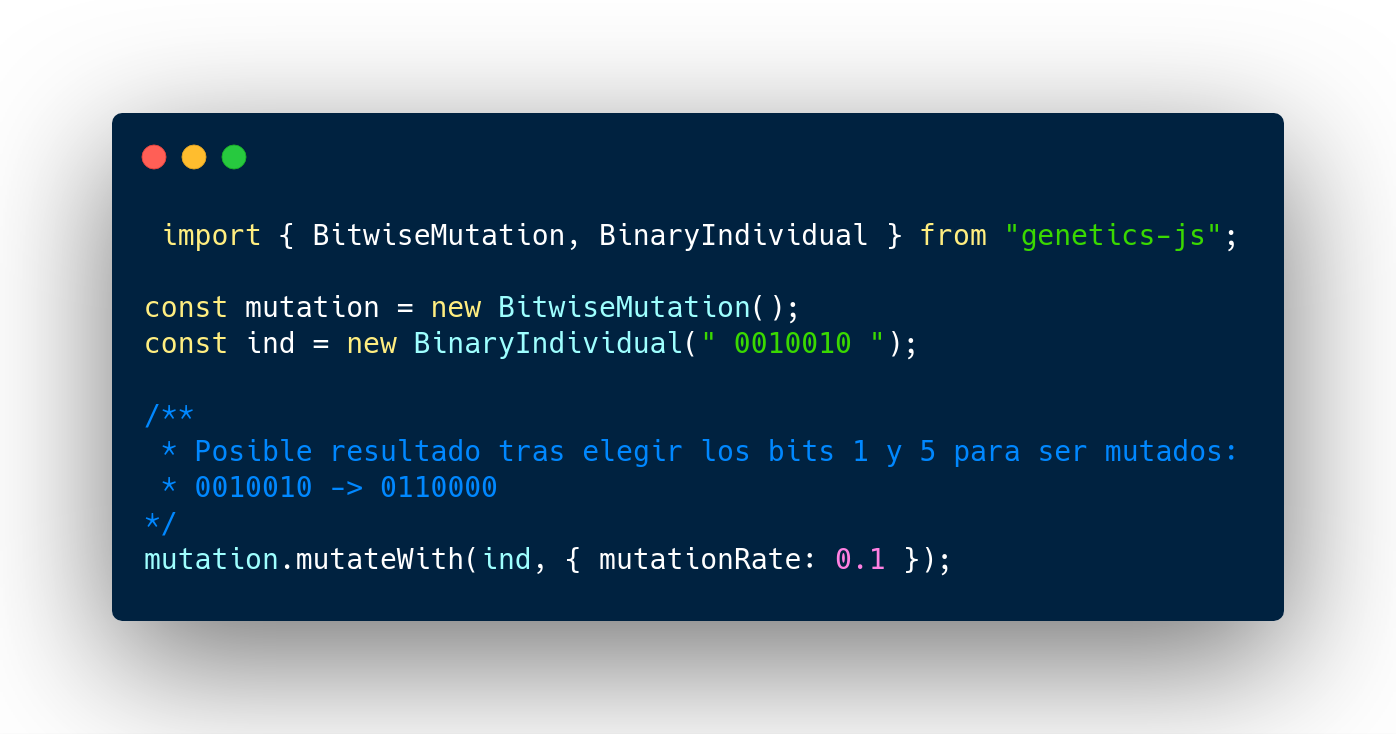
\includegraphics[scale=0.23]{pres/img/desarrollo/mutation-example.png}
    \caption{Ejemplo de una operación de mutación}
    \label{fig:my_label}
\end{figure}

\end{frame}
%++++++++++++++++++++++++++++++++++++++++++++++++++++++++++++++++++++++++++++++ 

%++++++++++++++++++++++++++++++++++++++++++++++++++++++++++++++++++++++++++++++ 
\begin{frame}
\frametitle{Reemplazo}

La fase de reemplazo consiste en determinar que individuos compondrán la siguiente generación teniendo a la población inicial y a la descendencia generada.

\bigskip

\begin{figure}
    \centering
    \subfloat{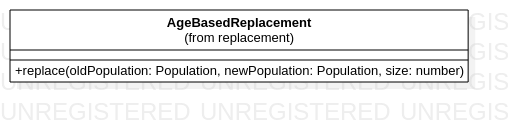
\includegraphics[scale=0.3]{mem/images/cap-4/4.2.8(Reemplazo)/AgeBasedReplacement.png}}
    \qquad
    \subfloat{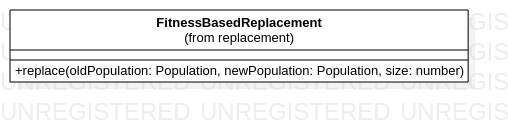
\includegraphics[scale=0.3]{mem/images/cap-4/4.2.8(Reemplazo)/FitnessBasedReplacement.png}}
    \caption{Diagramas de \texttt{AgeBasedReplacement} y \texttt{FitnessBasedReplacement}}
    \label{fig:1}
\end{figure}

Los métodos de selección implementados han sido:

\begin{itemize}
    \item \texttt{AgeBasedReplacement}
    \item \texttt{FitnessBasedReplacement}
\end{itemize}

\end{frame}
%++++++++++++++++++++++++++++++++++++++++++++++++++++++++++++++++++++++++++++++

%++++++++++++++++++++++++++++++++++++++++++++++++++++++++++++++++++++++++++++++ 
\begin{frame}
\frametitle{Puntuación (\textit{fitness})}

La función de puntuación (\textit{fitness}) se utiliza para determinar \textbf{cuanto de adaptado al medio} está el individuo que se pretende evaluar. En el caso de un problema de optimización, esta función se corresponde con la que se pretende optimizar.

\begin{center}
    \texttt{type FitnessFunction<I extends BaseIndividual<T>, T> = (individual: I) => number}
\end{center}

\begin{figure}
    \centering
    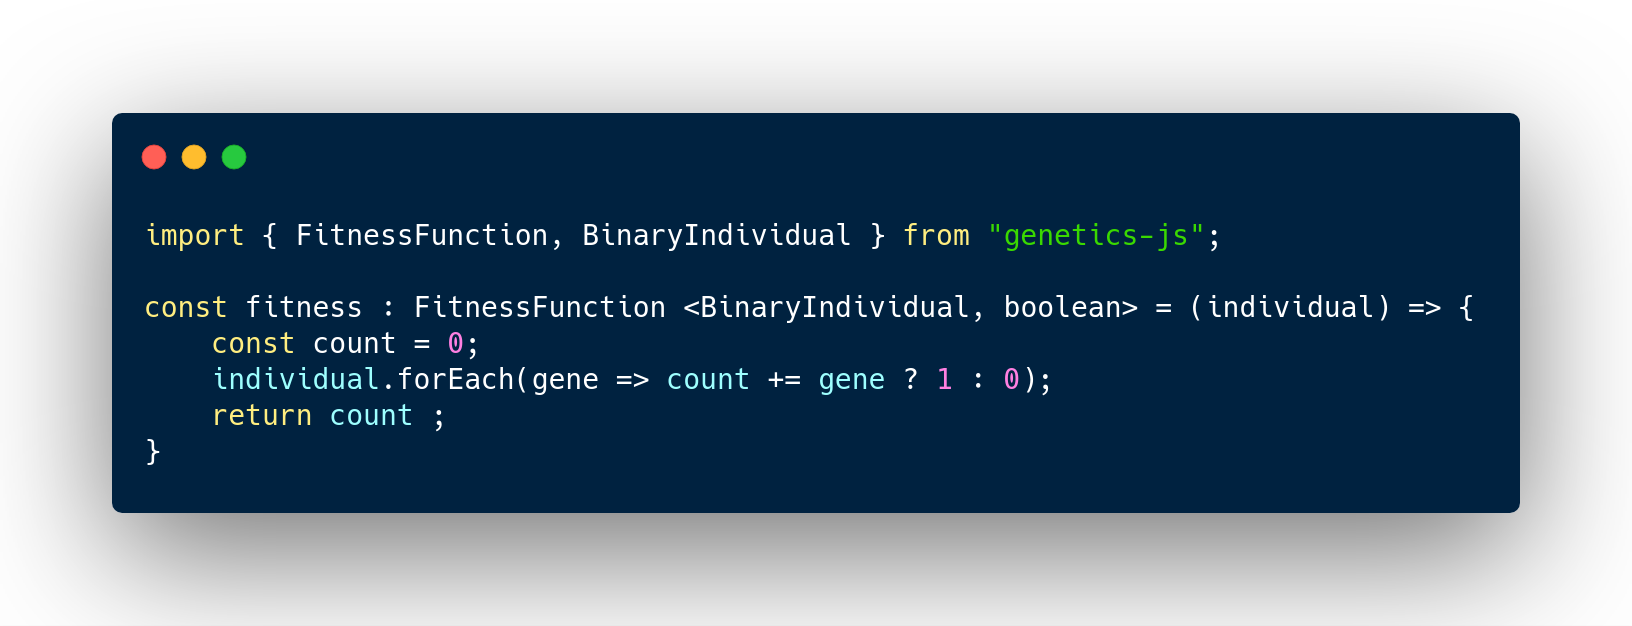
\includegraphics[scale=0.20]{pres/img/desarrollo/fitness-example.png}
    \caption{Ejemplo de una función de fitness}
    \label{fig:my_label}
\end{figure}

\end{frame}
%++++++++++++++++++++++++++++++++++++++++++++++++++++++++++++++++++++++++++++++

%++++++++++++++++++++++++++++++++++++++++++++++++++++++++++++++++++++++++++++++ 
\begin{frame}
\frametitle{Condición de finalización}

La condición de finalización es el criterio que determinará cuando se detendrá el algoritmo evolutivo. En este caso, \textbf{un número máximo de iteraciones sin mejora}.

\begin{figure}
    \centering
    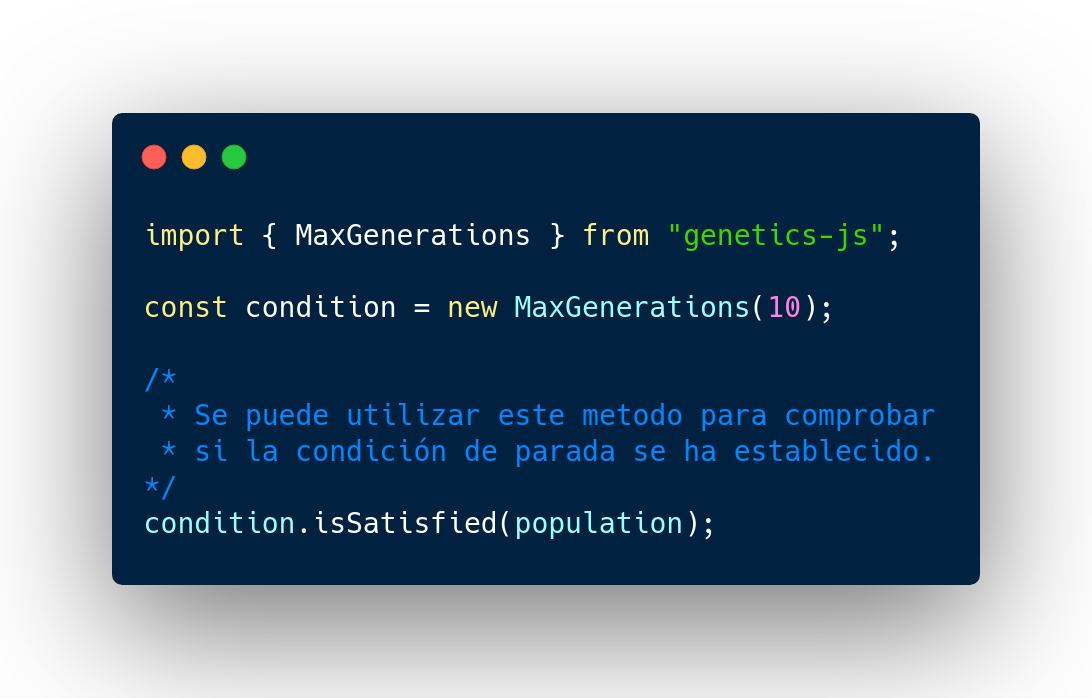
\includegraphics[scale=0.22]{pres/img/desarrollo/termination-example.png}
    \caption{Utilización de la condición de parada}
    \label{fig:my_label}
\end{figure}

\end{frame}
%++++++++++++++++++++++++++++++++++++++++++++++++++++++++++++++++++++++++++++++

\section{Ejemplo de uso}

%++++++++++++++++++++++++++++++++++++++++++++++++++++++++++++++++++++++++++++++ 
\begin{frame}
\frametitle{Ejemplo de uso}

Para el ejemplo de uso implementaremos una aplicación web con \textbf{React}, que permita resolver el problema de la mochila (\textbf{Knapsack Problem}).

\bigskip

\begin{columns}
    \column{0.4\textwidth}
    Formulación del problema:
    \begin{equation*}
        \begin{aligned}
        & \underset{X}{\text{max}}
        & & \sum_{i=1}^n v_i x_i \\
        & \text{sujeto a}
        & & \sum_{i=1}^n w_i x_i \leq W \\
        &&& x_i \in \{0, 1\}
        \end{aligned}
    \end{equation*}
    \column{0.6\textwidth}
    \begin{block}{Despliegue de la aplicación}
     \url{https://cristianabrante.github.io/GeneticsJsKnapsack/}
    \end{block}
\end{columns}

\end{frame}
%++++++++++++++++++++++++++++++++++++++++++++++++++++++++++++++++++++++++++++++

%++++++++++++++++++++++++++++++++++++++++++++++++++++++++++++++++++++++++++++++  
\end{document}
